\documentclass[a4paper,12pt]{article} 

%article 文档类型适合较短的文章,比如期刊文章和短篇报告。
%article 文档的正文会紧跟着标题之后在同一页上排版。report 会将标题置为单独的一页。
%其他文档类型包括 report(适用于更长的多章节的文档,比如博士生论文),
%proc(会议论文集),book 和 beamer。
%方括号内的文本指定了一些选项——示例中它设置纸张大小为 A4,主要文字大小为 12pt。

\usepackage{color}

\usepackage[UTF8]{ctex}%ctex 宏包用于支持中文排版,UTF8 选项指定了文档的编码格式为 UTF-8。
%ctex 宏包提供了对中文的支持,包括中文字体、段落格式等。如果不需要中文支持,可以删除这一行。

\usepackage{amsmath} %使用 amsmath 宏包来支持数学公式
%amsmath 宏包提供了对数学公式的支持,包括公式编号、对齐等。如果不需要数学公式支持,可以删除这一行。

\usepackage{graphicx} % 使用 graphicx 宏包来支持图形插入
%graphicx 宏包提供了对图形插入的支持,包括图形的缩放、旋转等。如果不需要图形插入支持,可以删除这一行。
\usepackage{float} % 使用 float 宏包来支持 [H] 选项

%\usepackage{hyperref} % 使用 hyperref 宏包来支持超链接
%hyperref 宏包提供了对超链接的支持,包括目录、引用等。如果不需要超链接支持,可以删除这一行。

%\usepackage{geometry} % 使用 geometry 宏包来设置页面布局
%geometry 宏包提供了对页面布局的支持,包括页边距、纸张大小等。如果不需要自定义页面布局,可以删除这一行。     

%\usepackage{fancyhdr} % 使用 fancyhdr 宏包来设置页眉页脚
%fancyhdr 宏包提供了对页眉页脚的自定义支持,包括页眉页脚的样式、内容等。如果不需要自定义页眉页脚,可以删除这一行。

%\usepackage{lipsum} % 使用 lipsum 宏包来生成示例文本
%lipsum 宏包提供了生成示例文本的功能,通常用于测试文档布局。如果不需要示例文本,可以删除这一行。

\begin{document}


\title{Latex使用指南}
\author{Xie Yuan}
\date{\today}
\maketitle % \maketitle 用于生成标题页,包含文档标题、作者和日期。

%使用 \tableofcontents 在文档中创建目录。通常我们会在标题的后面建立目录。
\pagenumbering{roman} % 设置页码格式为罗马数字
\tableofcontents % 创建目录
\pagenumbering{arabic} % 设置页码格式为阿拉伯数字

%\setlength{\parindent}{0pt}% % 设置段落缩进为0,全局形态
%section{...}表示一个章节的标题,通常用于文章的主要部分。

\listoftables % 创建表格目录 
\listoffigures % 创建图表目录   
\newpage % 换页
 

    \section{字体和颜色}

        \subsection{字体样式和颜色}
    
        {\color{red}\textit{This is the introduction section of my first document.}}
%{\color{colorname}text}用于将文本设置为红色。
%textit{...}用于将文本设置为斜体。
%textbf{...}用于将文本设置为粗体。
%texttt{...}用于将文本设置为等宽字体,通常用于代码或命令。
%textsc{...}用于将文本设置为小型大写字母。
%textsl{...}用于将文本设置为斜体,通常用于强调文本。
%emph{...}用于强调文本,通常会将文本设置为斜体。
%itemize 环境用于创建无序列表,enumerate 环境用于创建有序列表。
        \\ \colorbox{blue}{\indent textsl{ This section describes the methods used in this document.}}
%\colorbox{colorname}{textsl{...}}用于将文本设置为蓝色背景并斜体。
        \\ \underline{\indent This subsection discusses the second stage of the methods.}

        \subsection{字体大小}

        \paragraph{\indent normal size words {\tiny tiny words} {\scriptsize scriptsize words} 
        {\footnotesize footnotesize words} {\small small words} {\normalsize normal size words} 
        {\large large words} {\Large Large words} {\LARGE LARGE words} {\huge huge words} {\Huge Huge words}}


    \section{标签和段落}        
     
        \subsection{标签和引用}%subsection{...}表示一个子章节的标题,通常用于章节的细分。

        \label{sec1}This subsection discusses the first stage of the methods.
        \\ Here are your results. Referring to section \ref{sec1} on page \pageref{sec1}
%使用 \label{labelname} 对章节创建标签。
%然后输入 \ref{labelname} 或者 \pageref{labelname} 来引用对应的章节。
        
        \subsection{段落分级}
        
%paragraph{...}表示一个段落的标题,通常用于更小的细分
        \paragraph{\indent This is a paragraph.} %一般显示为顶格
            \subparagraph{This is a smaller paragraph.}
            %该代码一般缩进显示,subparagraph{...}表示一个子段落的标题,通常用于更小的细分。
    
    
    \section{字符使用} 
    
        \subsection{缩进和换行}%每个章节的首段都显示缩进
        This is a very part,and help ours understand the document.这将会帮助我们精心的理解文档。  
        \\ \indent{conclusion is important for a document,} % \\可以用来换行

        \vspace{1cm} % \vspace{1cm} 可以用来添加1厘米的垂直空白

        \indent{it summarizes the main points and findings.No one born being good at all things.}

        \subsection{特殊字符}
    
%在 LaTeX 中,某些字符有特殊含义,如 # $ % & _ { } ~ ^ \ 等。
%如果需要在文本中使用这些字符,可以使用反斜杠 \ 来  
%转义它们。例如,使用 \# 来表示井号 #,使用 \$ 来表示美元符号 $。
%如果需要在文本中使用反斜杠本身,可以使用 \text或者 \textbackslash 来表示。                    
        \#  \indent{\textbackslash} 
        \\ \indent{\$} % \indent 用于缩进 \noindent 用于取消段落缩进 
        \\ \indent{\^e}  \indent{\^{}e}
 % 注意在使用 ^ 和 ~ 字符的时侯需要在后面紧跟一对闭合的花括号,否则他们就会被解释为字母的上标.


    \section{图和表}

        \subsection{列表}
%itemize 环境用于创建无序列表,enumerate 环境用于创建有序列表。
        \begin{enumerate}
            \item[-] First item     %使用方括号参数来修改无序列表头的标志
       
            \item[+]Second thing
                \begin{itemize}
                    \item[Fish] A sub\_thing
            
                    \item[Plants] Another sub\_thing
                \end{itemize}

            \item[Q] Third item
        \end{enumerate}
    
        \subsection{表格}
    
%tabular 环境用于创建表格。LaTeX 默认表格是没有横向和竖向的分割线的,如果你需要,你得手动设定。LaTeX 会根据内容自动设置表格的宽度。
% \begin{tabular}{...} 省略号部分指定了列的对齐方式和分隔符。
% l>表示左对齐,c 表示居中对齐,r 表示右对齐。| 表示列之间有竖线分隔。
%{lll} 会生成一个三列的表格,并且保存向左对齐,没有显式的竖线.
%{|l|l|r|} 会生成一个三列表格,前两列左对齐,最后一列右对齐,并且相邻两列之间有显式的竖线。
% 表格的数据在 \begin{tabular} 后输入.  
% \begin{tabular}{|l|l|} %使用 |l|l| 来创建两列的表格,并且在列之间添加竖线分隔符
% & 用于分割列,\\ 用于分割行。
% \hline 用于添加整个表格横向分割线,\cline{1-2} 用于添加部分(一列和二列)横向分割线。
% \end{tabular} 用于结束表格环境。

        \begin{table}[H]
            \centering
            \begin{tabular}{|l|l|}
                Apples       & green \\
                Strawberries & red    \\
                Bananas      & yellow  \\
            \end{tabular}
            \caption{Here is my table1}
        \end{table}


        \begin{table}[H]
            \centering
            \begin{tabular}{rc}
                Apples                       &  green   \\
                \hline
                Strawberries                 &  red      \\
                \cline{1-1} Oranges          &  orange   \\
            \end{tabular}
            \caption{Here is my table2}
        \end{table}


       \begin{table}[H]
            \centering
            \begin{tabular}{|r|l|}
                \hline
                8                &  here`s   \\
                \cline{2-2} 86   &  stuff    \\
                \hline
                \hline
                2008             &   now     \\
                \hline
            \end{tabular}
            \caption{Here is my table3}
        \end{table}
    
        \begin{table}[H]
            \centering
            \begin{tabular}{l|r|r}
                Item             &   Quantity     &   Price(\$)     \\
                \hline
                Nails            &    500         &    0.34          \\
                Wooden boards    &    100         &    4.00          \\
                Bricks           &    240         &    11.50          \\
            \end{tabular}
            \caption{Here is my table4}
        \end{table}

        
        \begin{table}[H]
            \centering
            \begin{tabular}{l|ccc}
                      &      year                      \\
                \cline{2-4}
                City      &   2006    &   2007    &   2008   \\
                \hline
                London    &   45789   &   46551   &   51298   \\
                Paris     &   34549   &   32543   &   29870    \\
                New York  &   49835   &   51009   &   51970    \\
            \end{tabular}
            \caption{Here is my table5}
        \end{table}
        
        \subsection{图片} %注意图表的插入需要使用 graphicx 宏包。
        
        \begin{figure}[H] %[h] 选项表示图表将被放置在当前位置(here)。t表示放在页面顶端,b表示放在页面底端,p表示放在独立的页面上。!参数表示强制放置在指定位置。
            \centering    % \centering 用于将图表居中对齐,默认左对齐。
            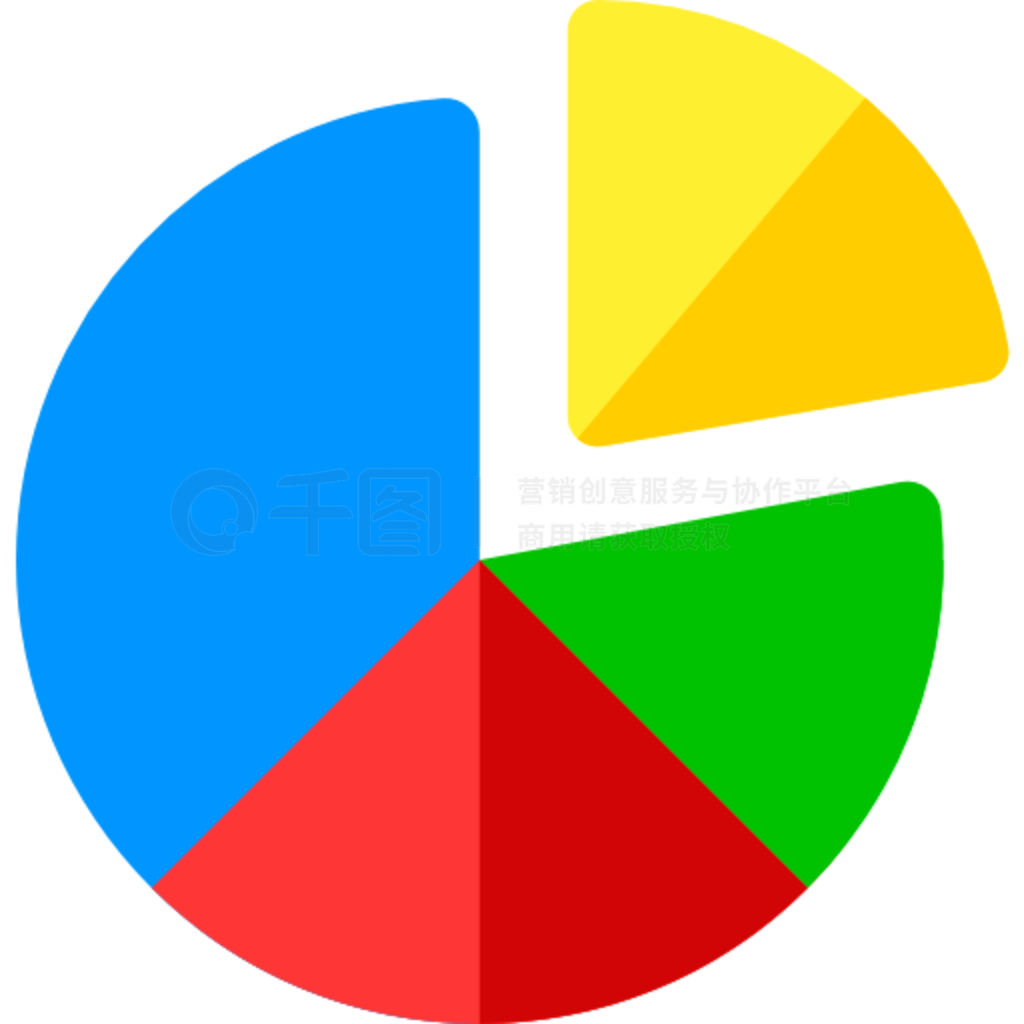
\includegraphics[width=0.3\textwidth]{1} %如果你的文件名有空格,就使用双引号包裹,比如 "screen 20"。
            %可以自动将图放置到你的文档中,图片文件应当与 TeX 文件放在同一目录下。
            %width=0.5\textwidth 表示图的宽度为文本宽度的一半。你可以根据需要调整这个比例。宽度也可以厘米为单位,
            %[scale=0.5] 表示图的大小为原来的 50%。你可以根据需要调整这个比例。
            %如果你需要旋转图像,可以使用 [angle=90] 选项
            %\includegraphics[angle=90]{image.png} 将图像旋转90度。
            %如果你需要裁剪图像,可以使用 [trim=left bottom right top] 选项
            %\includegraphics[trim=1cm 2cm 1cm 2cm]{image.png} 将图像裁剪掉左边1厘米、底部2厘米、右边1厘米和顶部2厘米的部分。
            %\includegraphics[opacity=0.5]{image.png} 将图像的透明度设置为 50%。
            \caption{Here is my image} %定义图表的标题,如果使用了它,LaTeX 会给你的图表添加「Figure」开头的序号。用 \listoffigures 来生成一个图表的目录。
            \label{image-1} %使用 \label{labelname} 来创建标签,之后可以使用 \ref{labelname} 来引用图表。
        \end{figure}
        
         This is a reference to 图 \ref{image-1} on page \pageref{image-1}.

    
    \section{数学公式}

        \subsection{插入公式}
        %数学公式可以使用 $...$ 或者 \begin{equation} ... \end{equation} 来插入。
        %$...$ 用于行内公式,\begin{equation} ... \ end{equation} 用于独立公式。
        %行内公式会与文本在同一行显示,而独立公式会单独成行显示。
        %如果你想要行间的公式,可以使用 $$...$$(现在我们推荐使用 \[...\],因为前者可能产生不良间距)
        %如果需要编号公式,可以使用 \begin{equation} ... \end{equation},LaTeX 会自动为公式添加编号。
        %如果不需要编号公式,可以使用 \begin{equation*} ... \end{equation*}。
        %如果需要对齐多个公式,可以使用 \begin{align} ... \end{align},LaTeX 会自动对齐公式。
        %如果需要对齐多个公式并且编号,可以使用 \begin{align} ... \end{align},LaTeX 会自动对齐公式。
        
        这是一个行内公式,$1+2=3$ 与文本在同一行显示。
        \\ \indent 这是一个行间公式,$$1+2=3$$   \indent 与文本在同一行显示。

        \vspace{1cm}

        \indent 这是一个独立公式:
            \begin{equation*}
                1+2=3
            \end{equation*}
    
            \begin{eqnarray*}
                a & =& b + c \\
                & = & y - z
            \end{eqnarray*}

            \begin{align*}
               a^2 + b^2 &= c^2 \\
               x^2 + y^2 &= z^2
            \end{align*}
        
        \subsection{数学符号}
            
            \subsubsection{上标和下标}

            上标(Powers)使用 \texttt{\^} 来表示,比如 $n^2$
            \\ \indent 下标(Indices)使用 \_ 表示,比如 $2_{a}$
            \\ \indent  包含上标和下标的公式使用 \{ \} 来包裹,比如 $b_{a-2}$
        
            \subsubsection{分数}
            分数用\textbackslash frac\{numerator\}\{denominator\} 来表示,比如\textbackslash frac\{a\}\{b\}表示 $$\frac{a}{b}$$
            \\分数可以嵌套,比如 \textbackslash frac\{y\}\{\textbackslash frac\{3\}\{x\}+b\}表示为$$\frac{y}{\frac{3}{x}+b}$$
        
            \subsubsection{根号}

            我们使用 \textbackslash sqrt\{...\} 插入根号,省略号的内容由被开根的内容替代。
            \\ \textbackslash sqrt\{$a^2$\}的结果是 $$\sqrt{a^2}$$
            \\  \indent 如果需要添加开根的次数,使用方括号括起来即可。
            \\ \textbackslash sqrt[x]\{$y^2$\}的结果是 $$\sqrt[x]{y^2}$$
        
            \subsubsection{求和和积分}
             
            使用 \textbackslash sum 和 \textbackslash int 来表示求和和积分。上限使用\^{},下限使用\_{}
            \\ \textbackslash sum\_\{x=1\} y\^{}z 的结果是 $$\sum_{x=1}^5 y^z$$
            \\ \textbackslash int\_a\^{}b f(x) 的结果是 $$\int_a^b f(x)$$

            \subsubsection{希腊字母}
           
            使用反斜杠加希腊字母的名称来表示一个希腊字母,名称的首字母的大小写决定希腊字母的形态。
            \\ \indent \textbackslash alpha = $\alpha$
            \\ \indent \textbackslash bate = $\beta$
            \\ \indent \textbackslash delta \textbackslash Delta = $\delta$ $\Delta$
            \\ \indent \textbackslash pi \textbackslash Pi = $\pi$ $\Pi$
            \\ \indent \textbackslash sigma \textbackslash Sigma = $\sigma$ $\Sigma$
            \\ \indent \textbackslash omega \textbackslash Omega = $\omega$ $\Omega$
      
            
    \section{参考文献} 
        \subsection{手动添加参考文献}
        你可以使用 thebibliography 环境来手动添加参考文献。
        \\ \indent 使用 \textbackslash begin\{thebibliography\}\{99\} 来开始参考文献环境,99 是参考文献的最大编号。
        \\ \indent 使用 \textbackslash bibitem\{labelname\} 来添加一条参考文献,labelname 是该参考文献的标签名称。
        \\ \indent 使用 \textbackslash end\{thebibliography\} 来结束参考文献环境。
        \\ \indent 使用 \textbackslash cite\{labelname\} 来引用参考文献,labelname 是该参考文献的标签名称。
        
        这是一个引用参考文献的例子 \cite{leslie}。

        \begin{thebibliography}{99}
            \bibitem{leslie} Leslie Lamport. LaTeX: A Document Preparation System. Addison-Wesley, 2nd edition, 1994.
            \bibitem{frank} Frank Mittelbach and Michel Goossens. The LaTeX Companion. Addison-Wesley, 2nd edition, 2004.
            \bibitem{donald} Donald E. Knuth. The TeXbook. Addison-Wesley, 1986.
        \end{thebibliography}  

        \subsection{插入文献列表}
        \indent 首先,你需要创建一个 .bib 文件,里面包含你的参考文献条目。
        \\ \indent 然后,在你的主 .tex 文件中,使用 \textbackslash bibliography\{filename\} 来指定你的 .bib 文件,filename 是你的 .bib 文件的名称(不包含扩展名)。
        \\ \indent 使用 \textbackslash bibliographystyle\{style\} 来指定参考文献的样式,style 是你选择的样式名称,比如 plain、abbrv、alpha 等。
        \\ \indent 使用 \textbackslash cite\{labelname\} 来引用参考文献,labelname 是该参考文献的标签名称。 
        
        
        \subsection{参考文献标注}
        \indent 使用 \textbackslash cite\{citationkey\} 来在你想要的引用文献的地方插入一个标注,
        \indent 如果你不希望在正文中插入一个引用标注,但仍想要在文献列表中显示这次引用,使用 \textbackslash nocite\{citationkey\}。
        \indent 如果你想要在引用中插入页码信息,使用方括号:\textbackslash cite[p. 123]\{citationkey\}。
        \indent 如果你想要引用多个文献,使用逗号分隔:\textbackslash cite\{citation1,citation2,citation3\}。
        

        \subsection{引用格式}
            \subsubsection{数字标号引用}
            LaTeX 包含了多种行内数字标号引用的格式:
            \\ \indent Plain 方括号包裹数字的形式,如 [1] 。文献列表按照第一作者的字母表顺序排列。每一个作者的名字是全称。
            \\ \indent Abbrv 与 plain 是相同的,但作者的名字是缩写。
            \\ \indent Unsrt 与 plain 是相同的,但文献列表的排序按照在文中引用的先后顺序排列。
            \\ \indent Alpha 与 plain 一样,但引用的标注是作者的名字与年份组合在一起,不是数字,如 [Kop10]。   
            
            \subsubsection{作者日期引用}
            如果你想使用作者日期的引用,使用 natbib 包。
            \\ \indent 使用\textbackslash \{...\}命令来生成一个方括号标注,如[Koppe,2010].
            使用\textbackslash citet\{...\}来生成一个标注,来生成一个标注,只把年份放到方括号里,如 Koppe [2010]
            \\ \indent Natbib包也有三种格式:plainnat,abbrvnat 和 unsrtnat,他们与 plain,abbrv 和 unsrt 的效果是一样的。

            \subsubsection{其他引用格式}
            如果你需要使用不同的格式,你需要在同一个文件夹下创建一个格式文件(.bst 文件)。
            \\ 引用这个格式的时侯使用它的文件名调用 \textbackslash bibliographystyle{...} 命令实现。
\end{document}